\section{高斯信道}
\label{sec:gcc-channel}

第~\ref{chap:discrete-channel-capacity}章的信道只有有限个输入和输出。线路上实际传送的常常是一个连续的幅值，例如一个电压；接收端读到的是这个幅值加上一份随机扰动。扰动通常是许多微小独立因素的叠加，由第~\ref{chap:central-limit-theorem}章的中心极限定理，用高斯分布描述它是自然的近似。这一节先写清模型和编码的规则，再说明为什么必须限制输入的功率，最后用几何图景猜出容量公式。

\paragraph{加性高斯噪声模型}
输入、输出都取实数值，每次使用信道，输出等于输入加上一个独立的高斯噪声。

\begin{definition}[高斯信道]
\label{def:gcc-channel}
设$\sigma^2>0$。\term{高斯信道}（Gaussian channel）在第$i$次使用时把实数输入$x_i$变成输出
\begin{equation}
 Y_i=x_i+Z_i,\qquad i=1,\dots,n,
 \label{eq:gcc-channel}
\end{equation}
其中$Z_1,\dots,Z_n$独立同分布，$Z_i\sim\mathcal{N}(0,\sigma^2)$，并且与要传送的消息、与编码器选出的输入相互独立。
\end{definition}

记$g_v$为$\mathcal{N}(0,v)$的密度，
\begin{equation}
 g_v(t)=\frac{1}{\sqrt{2\pi v}}\exp\Bigl(-\frac{t^2}{2v}\Bigr),\qquad v>0 .
 \label{eq:gcc-gauss-density}
\end{equation}
给定输入块$x^n=(x_1,\dots,x_n)$，输出块$Y^n$的条件密度是各坐标密度之积，
\begin{equation}
 p(y^n\mid x^n)=\prod_{i=1}^{n}g_{\sigma^2}(y_i-x_i) .
 \label{eq:gcc-block-density}
\end{equation}
这就是第~\ref{chap:discrete-channel-capacity}章无记忆性的连续版本：转移矩阵的乘积换成了条件密度的乘积，各次使用的噪声互不影响。条件密度的含义取自第~\ref{chap:conditional-distributions}章。

与离散信道相比，有两处不同。第一，输入字母表是整条实轴，不能在有限个分布的单纯形上做优化；第二，任意两个输入都可能产生同一个输出，输出不会只落在有限个位置上。图~\ref{fig:gcc-channel-model}画出整块传输的过程。

\begin{BookInlineFigure}
 \centering
 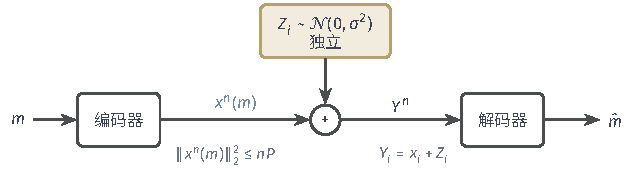
\includegraphics[width=107mm]{figures/07-probability/06-channel-coding/tikz/gcc-channel-model/figure.pdf}
 \caption{高斯信道上的块传输。编码器把消息$m$映成实数码字$x^n(m)$（蓝），它的能量不超过$nP$；每个坐标加上独立的噪声$Z_i\sim\mathcal{N}(0,\sigma^2)$（黄框），解码器根据输出块$Y^n$判决$\hat{m}$。}
 \label{fig:gcc-channel-model}
\end{BookInlineFigure}

\paragraph{不限制幅值时}
先看单次使用、只发两种消息的情形。发送$+A$或$-A$，接收端看输出的符号：输出为正判为$+A$，否则判为$-A$。发送$+A$而判错，需要噪声小于$-A$，概率是
\[
 \mathbb{P}(Z<-A)=\Phi\Bigl(-\frac{A}{\sigma}\Bigr) ,
\]
其中$\Phi$是标准高斯分布函数。取$\sigma=1$，$A=1$时这个概率是$0.159$，$A=3$时降到$0.00135$。图~\ref{fig:gcc-two-point}画出两种情形下的两条输出密度：幅值越大，两条钟形分得越开，重叠的尾部越小。

\begin{BookInlineFigure}
 \centering
 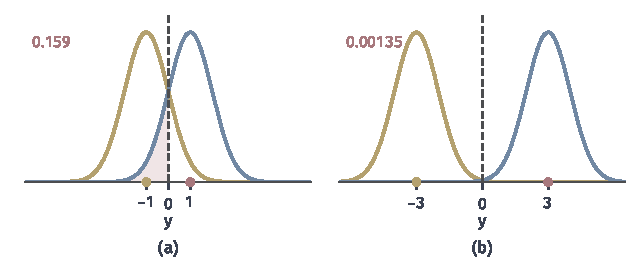
\includegraphics[width=108mm]{figures/07-probability/06-channel-coding/matplotlib/gcc-two-point/figure.pdf}
 \caption{两点输入$\pm A$经过$\sigma^2=1$的高斯噪声。黄线是发送$-A$时的输出密度，蓝线是发送$+A$时的输出密度，虚线是判决门限$0$，红色阴影是发送$+A$而判错的概率。(a)$A=1$，错误概率$0.159$。(b)$A=3$，错误概率$0.00135$。}
 \label{fig:gcc-two-point}
\end{BookInlineFigure}

幅值不受限制时，可靠传输没有上限。把间距固定为$d$，在实轴上放$K$个等距的输入点，每个点被判错的概率不超过$2\Phi(-d/(2\sigma))$，只要$d$足够大，这个概率可以任意小，而$K$可以任意大。于是每次使用可以近乎无错地送出$\log_2K$比特，$K$没有上界。同理，若$\sigma^2=0$，任意两个不同的实数都能被区分，一次使用就能送出任意多的比特。所以有意义的问题必须同时有两个前提：噪声方差为正，输入的幅值受到预算约束。

\paragraph{功率约束下的块码}
实际的发射设备受能量或平均功率的限制。约束加在每一条码字上：

\begin{definition}[功率约束下的块码]
\label{def:gcc-code}
设$P\geq0$。高斯信道上满足\term{功率约束}（power constraint）$P$的$(M,n)$码由编码器$f:\{1,\dots,M\}\to\mathbb{R}^n$与可测的解码器$g:\mathbb{R}^n\to\{1,\dots,M\}$组成，码字$x^n(m)=f(m)$对每条消息都满足
\begin{equation}
 \lVert x^n(m)\rVert_2^2=\sum_{i=1}^{n}x_i(m)^2\leq nP,\qquad m=1,\dots,M .
 \label{eq:gcc-power}
\end{equation}
\end{definition}

码率、条件错误概率、平均错误概率、最大错误概率和可达速率都沿用第~\ref{chap:discrete-channel-capacity}章的定义，只是把对输出块的求和换成对条件密度~\eqref{eq:gcc-block-density}的积分：
\begin{equation}
 \lambda_m=\int_{\{y^n:\,g(y^n)\neq m\}}p\bigl(y^n\mid x^n(m)\bigr)\,\mathrm{d}y^n ,
 \qquad P_{\mathrm{e}}=\frac1M\sum_{m=1}^{M}\lambda_m .
 \label{eq:gcc-errors}
\end{equation}
称$R$为功率$P$下的可达速率，若存在一列满足功率约束$P$的$(M_n,n)$码，$M_n\geq2^{nR}$且$P_{\mathrm{e}}\to0$。可达速率的上确界记作$C_{\mathrm{op}}(P)$。本章用$P$表示功率；分布写作带下标的$P_X$，概率写作$\mathbb{P}$，平均错误概率写作$P_{\mathrm{e}}$，三者不会混淆。

约束~\eqref{eq:gcc-power}有三点需要读清。

第一，它是沿一条码字的时间平均：$\frac1n\sum_ix_i(m)^2\leq P$。同一条码字可以在某些位置用大幅值、在另一些位置用小幅值，只要总能量不超预算。

第二，它对每一条码字分别成立，不允许一条码字超支、由另一条码字的节省来补偿。若只要求$\frac1M\sum_m\lVert x^n(m)\rVert_2^2\leq nP$，约束就变弱了。第~\ref{sec:gcc-coding}小节的逆定理说明，即使在这种较弱的约束下，速率也不能超过同一个上限。

第三，它是第~\ref{chap:discrete-channel-capacity}章输入成本约束的连续类比：成本函数取$c(x)=x^2$，预算取$\Gamma=P$。不同的是输入字母表不再有限，那里依赖有限单纯形紧性的论证都要重做。

$P=0$时，每条码字只能是零向量，不同消息的码字相同，只有$M=1$的码能做到无错，所以$C_{\mathrm{op}}(0)=0$。下文讨论容量公式时通常假设$P>0$，并在结论中注明端点。

\paragraph{噪声向量的长度}
把整块输出看成$\mathbb{R}^n$中的一个点，可以得到一幅几何图景。先看噪声向量$Z^n$的长度。由于$Z_i^2$独立同分布，期望为$\sigma^2$，第~\ref{chap:laws-of-large-numbers}章的弱大数律给出
\[
 \frac1n\lVert Z^n\rVert_2^2=\frac1n\sum_{i=1}^{n}Z_i^2\xrightarrow{\mathbb{P}}\sigma^2 .
\]
也就是说，块长很大时噪声向量的长度几乎总接近$\sqrt{n\sigma^2}$：$n$维高斯噪声集中在一个薄球壳上，而不是均匀地填满一个球。

图~\ref{fig:gcc-noise-norm}画出$\sigma^2=1$时$\lVert Z^n\rVert_2^2/n$的精确密度，它是$\chi^2_n$分布除以$n$。$\lVert Z^n\rVert_2^2/n$落在$[0.8,1.2]$中的概率，$n=4$时是$0.217$，$n=32$时是$0.579$，$n=256$时是$0.976$。

\begin{BookInlineFigure}
 \centering
 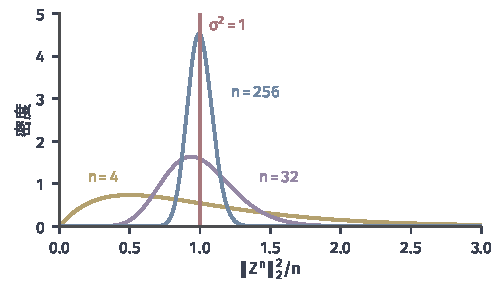
\includegraphics[width=84mm]{figures/07-probability/06-channel-coding/matplotlib/gcc-noise-norm/figure.pdf}
 \caption{$\sigma^2=1$时噪声向量的平均平方长度$\lVert Z^n\rVert_2^2/n$的密度，即$\chi^2_n/n$。黄、紫、蓝三条曲线分别对应$n=4,32,256$，红线是$\sigma^2=1$。块长越大，长度越集中在$\sqrt{n\sigma^2}$附近。}
 \label{fig:gcc-noise-norm}
\end{BookInlineFigure}

输出向量也有同样的现象。设码字满足$\lVert x^n\rVert_2^2\approx nP$，则
\[
 \frac1n\lVert x^n+Z^n\rVert_2^2=\frac1n\lVert x^n\rVert_2^2+\frac2n\langle x^n,Z^n\rangle+\frac1n\lVert Z^n\rVert_2^2 .
\]
中间的交叉项均值为零，方差为$4\sigma^2\lVert x^n\rVert_2^2/n^2\leq4\sigma^2P/n$，随$n$增大而趋于零；最后一项趋于$\sigma^2$。所以输出几乎总落在半径约$\sqrt{n(P+\sigma^2)}$的球内。

\paragraph{球的计数}
现在可以粗略地数一数能区分多少条消息。每条码字的输出集中在以码字为中心、半径约$\sqrt{n\sigma^2}$的小球附近；所有输出都在半径约$\sqrt{n(P+\sigma^2)}$的大球内。要从输出唯一认出码字，各个小球应当基本不重叠，于是码字数至多约为两球体积之比：
\[
 \frac{\bigl(\sqrt{n(P+\sigma^2)}\bigr)^{n}}{\bigl(\sqrt{n\sigma^2}\bigr)^{n}}
 =\Bigl(1+\frac{P}{\sigma^2}\Bigr)^{n/2} .
\]
这里用到了$n$维球的体积与半径的$n$次方成正比，比例常数在两球之间消去。取以2为底的对数再除以$n$，每次使用至多约送出
\[
 \frac12\log_2\Bigl(1+\frac{P}{\sigma^2}\Bigr)\ \text{比特}.
\]

全章的标量例子取$\sigma^2=1$，$P=3$。两球半径之比是$\sqrt{4}=2$，$n$维体积之比是$2^n$，每次使用约$1$比特。图~\ref{fig:gcc-sphere-packing}在平面上画出这幅图景；为了画得下，图中取$P/\sigma^2=8$。

\begin{BookInlineFigure}
 \centering
 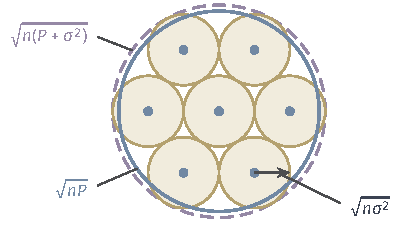
\includegraphics[width=68mm]{figures/07-probability/06-channel-coding/tikz/gcc-sphere-packing/figure.pdf}
 \caption{球的计数在平面上的示意（$n=2$，$P/\sigma^2=8$）。蓝点是码字，位于半径$\sqrt{nP}$的蓝色圆内；黄色小圆是半径$\sqrt{n\sigma^2}$的噪声球；所有输出落在半径$\sqrt{n(P+\sigma^2)}$的紫色虚线圆内。两圆面积之比是$9$，图中放下了$7$个互不重叠的噪声球。}
 \label{fig:gcc-sphere-packing}
\end{BookInlineFigure}

这个计数是启发，不是证明。体积之比只给出码字数的上限的猜测：它没有说明小球能否真的几乎不重叠地排满大球，也没有处理输出落在小球之外的情形。平面上的排列已经显示圆不能恰好铺满，图中$7$个小球只占大圆面积的$7/9$。下一节不再直接排列小球，而是先在单次使用上求互信息的最大值，再用随机选取的码字证明这个值可达；结果与上面的猜测一致。
